% LAB Final: Phonebook Project
%
% CSE/IT 107: Introduction to Programming
% New Mexico Tech
%
% Prepared by Christopher Koch, Hugo Rivera and Russell White
% Spring 2016
\documentclass[11pt]{cselabheader}

%%%%%%%%%%%%%%%%%% SET TITLES %%%%%%%%%%%%%%%%%%%%%%%%%
\fancyhead[R]{Final Project: Tanks}
\title{Final Project: Tanks}

\begin{document}

\pagenumbering{arabic}

\maketitle
\pagenumbering{roman}
\hrule

\begin{quotation}
  ``TANK TANK TANK''
\end{quotation}
\begin{flushright}
  --- Intro to \emph{Tank! Tank! Tank!}, Bandai Namco
\end{flushright}

\begin{figure}[H]
\centering
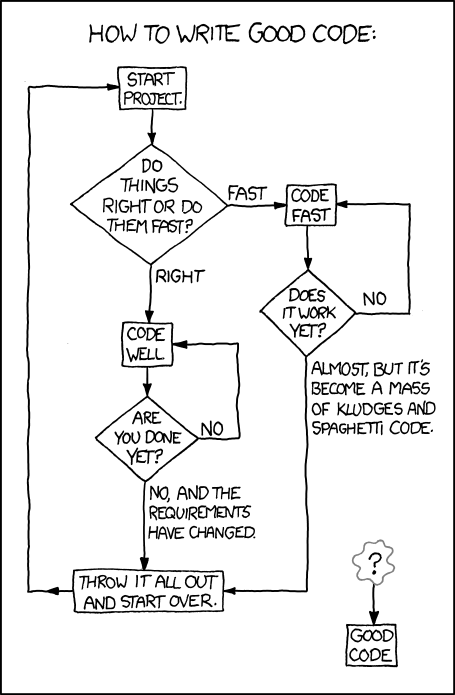
\includegraphics[width=0.5\textwidth]{img/xkcd_good_code.png}
\caption{XKCD on how to write good code \url{https://xkcd.com/844/}.}
\end{figure}

\hrule

\pagebreak
\tableofcontents

\begin{figure}[H]
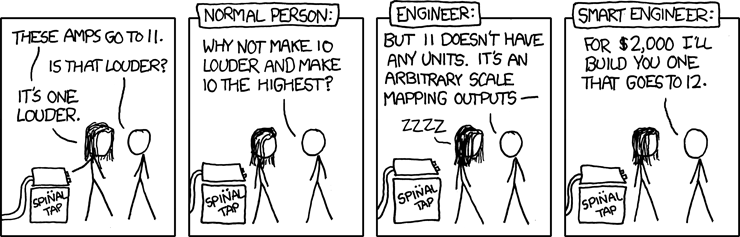
\includegraphics[width=\textwidth]{img/xkcd_spinal_tap_amps.png}
\caption{XKCD on engineers \url{https://xkcd.com/670/}.}
\end{figure}

\pagebreak
\pagenumbering{arabic}


\section{The Problem}

This project involves the modification of a skeleton of a game
involving several tanks.  You will complete the game, record the
interactions between tanks and plot this data using Matplotlib.

\subsection{Given Code}

The game currently consists of the files \texttt{game.py},
\texttt{sample\_tank.py}, \texttt{sensor.py}, \texttt{tank.py}, and
\texttt{tankutil.py}. For a description of what each of these files
do.

\subsubsection{main.py}
\texttt{main.py} contains the \pythoninline{main()} function of the program.
You will need to modify this file in order to add your own tanks to the
\pythoninline{Game} instance that is already being created. To do this,
simply imitate how the \pythoninline{SampleTank}s are being added. Note
that you will also need to add an import at the start of the file in
order to be able to access your tanks from other files.

\subsubsection{game.py}
\texttt{game.py} contains \pythoninline{class Game}. \pythoninline{Game}
contains the code that controls the interaction between tanks (collision
detection and firing) as well as the drawing of objects to the
\pythoninline{tkinter} window. You should not have to worry about how it does
these things and should not edit this file.

\subsubsection{tank.py}
\texttt{tank.py} contains \pythoninline{class Tank}, which includes all the
methods and attributes needed for general functionality of tanks. All of your
custom tanks should inherit from \pythoninline{Tank}. \emph{You should not edit
this file whatsoever.} Each tank has a large collection of attributes that
control its behavior. Most of these you should not touch, but for some of the
required tanks you may need to change the values of specific attributes in
your custom constructor.

For your tanks, you will need to redefine
\pythoninline{ai(self, delta)}, which is the method called each simulation step
to determine what the tank should do. Inside of this method, the only other
methods you should call are those in the section of \texttt{tank.py} labeled
``\texttt{METHODS TO BE USED BY AI}''. They allow you to set the desired speed
of the tank treads, the desired angle of the turret, and whether the tank should
fire. They also allow you to check the current status of the treads, turret, and
the sensors (described in Section\ref{subsubsec:sensor}). Not using these
methods will result in your tank not behaving properly, as properties such as
tread acceleration, max speed, and turret speed may be ignored.

You should also redefine \pythoninline{__init__} to specify the tank's sensors as
well as any other attributes that may differ from the default tank (left to your
discretion).

\subsubsection{tankutil.py}
\texttt{tankutil.py} contains a few miscellaneous functions used by the other
files. It is relatively inconsequential and you won't need to use it, though it
may be useful to look at if you want to set custom colors for your tanks. Once
again, you should not edit this file.

\subsubsection{sensor.py}
\label{subsubsec:sensor}
\texttt{sensor.py} contains \pythoninline{class Sensor}, which is used to define
the sensors for tanks. \pythoninline{Sensor} contains nothing but a constructor
and a few attributes. The actual logic for sensors resides inside
\texttt{game.py}.

A sensor is defined from four attributes:
\begin{description}
\item[Direction] A value in degrees that determines what direction the sensor
    is facing. This direction will indicate the middle of the sensor. 0 means
    directly in front of the tank, while 180 means directly behind the tank.
\item[Width] A value in degrees that determines how wide the sensor is. The
    sensor will detect tanks in half this number of degrees in each direction
    from the direction chosen above.
\item[Size] How far the sensor reaches. This distance is in pixels. For
    reference, the default range of a tank's gun is 50.
\item[Tracking] Whether or not the sensor will move as the gun's turret moves.
    This value should be either \pythoninline{True} or \pythoninline{False}. If
    this value is \pythoninline{False}, then the sensor's direction will be
    relative to the tank's current facing. If this value is \pythoninline{True},
    then the sensor's direction will be relative to the turret. This allows you
    to have sensors that, for example, check if there is something to the left
    or right of the turret that could be shot if the turret was moved slightly.
\end{description}

The sensors for your custom tanks should be created inside of the tank's
constructor. To check whether the sensor has detected a tank, use
\pythoninline{self.read_sensor(num)}, where \texttt{num} is the index of the
sensor inside of \pythoninline{self.sensors}.

Each sensor will be shown graphically, and if it detects a tank then it will be
filled in with the color of its parent tank to indicate that it is active.

As with \texttt{game.py}, \texttt{tank.py}, and \texttt{tank\_util.py} you should
not edit this file.


\subsubsection{sample\_tank.py}
\texttt{sample\_tank.py} is an example of how you might go about making your own
custom tanks. You are free to edit this file, but your final submissions should
be in separate files (as described in Section~\ref{subsec:ex}).
\pythoninline{class SampleTank} defines two methods: \pythoninline{__init__} and
\pythoninline{ai(self, delta)}. \pythoninline{__init__} is be used to
define two sensors: one large one that looks for anything in front of the tank
and one smaller one that follows the turret to check for anything that can be
shot. It also determines whether the turret will turn clockwise or
counter-clockwise.

\pythoninline{ai} is used to control the tank's behavior. The first thing this
tank does is get the current angle of the turret, then set the desired angle to
be higher or lower, depending on what chosen in the constructor. This results
in the turret continuously turning in one direction at a constant rate.

Next, the turret reads from sensor 1 and checks if the turret is able to fire.
Sensor 1 is the smaller sensor that is following the turret. If both values are
true, then the turret fires.

Finally, sensor 0 is checked. This is the large one in front of the tank. If
anything is detected, the tank reverses. If not, it continues forward, with the
left tread at a slightly higher speed than the right one. This results in the
tank slowly turning to the right.

\subsection{Bug Bounty}
The provided code may have some bugs.  As such, if you report a bug
that was not previously known, you will be given 5 points of extra
credit. If you can provide a \emph{fix} to a bug, you will be given 10
points. Report all bugs/fixes to your TA if you want to receive
credit.

\section{Assignment}
\label{subsec:ex}
You will be submitting 6 tanks that inherit from the \pythoninline{Tank} class
in \texttt{tank.py}. Each of your tanks should override, at the very least,
the \pythoninline{__init__} and \pythoninline{ai(self, delta)} methods of
the parent class.

You will be graded primarily on code quality, so remember to follow PEP-8 and
to document everything! Each tank file should give an overview of how its logic
works and why you made it work that way.

\subsection{Documentation}
\begin{ex}[README.txt]
You should have a README file briefly describing the logic behind each of your
tanks. If you changed anything in the given files besides the main() of
\texttt{main.py}, mention it here and explain why. Mention some changes you
found that made tanks more or less successful.

%%% Brief summary of your interactions analysis
\end{ex}

\subsection{Create Tanks}
\begin{ex}[coward.py]
This tank is nervous and doesn't like social interaction. It should do its best
to avoid all interaction with other tanks and evade them as much as possible.
Remember, this means more than simply going backwards if something is in front
of it -- think about what your tank should do if there's one tank in front of it
and another behind it!
\end{ex}

\begin{ex}[charger.py]
This tank is very enthusiastic to show you how well its turret works! It should
chase down any tank it sees and give them a demonstration of how good it is at
shooting things!\footnote{By shooting them.} If the gun isn't ready, it should
try to stay away from others so as not to reveal that its gun is not completely
reliable.
\end{ex}

\begin{ex}[turret.py]
This tank got its treads stuck in the mud. It should never move at all and
should move its turret, shooting anyone who comes near. It should also attempt
to track tanks as they approach if there isn't anyone currently in range to be
shot at.
\end{ex}

\begin{ex}[elephant.py]
The Elephant is a new experimental heavily armored tank. It is far slower and
larger than the other tanks while also being harder to kill.

To accomplish this, you will need to change some of the default tank attributes,
namely shape, radius, tread\_accel, and tread\_max. You will also need to
redefine \pythoninline{damage(self)}, which is called whenever a tank is shot
or runs into another tank.
\end{ex}

\begin{ex}[mouse.py]
The Mouse is a new experimental hyper fast tank. It is far more agile and
petite than the other tanks, attempting to succeed by dodging around other
tanks.

Similarly to with the Elephant, you will need to change some of the default tank
attributes.
\end{ex}

\begin{ex}[custom.py]
Finally, design your own custom tank that works however you wish. Try to give it
an AI that lets it combine the strategies of the other tanks in a way the makes
it better than all of them!
\end{ex}

\subsection{Analyze Behavior}
\begin{ex}[...]
%%% Use default game.py setup: arguments -> several different scenarios
%%% Record interactions somewhere... inherit from game.py?
\end{ex}

\begin{ex}[plot\_interactions.py]
\end{ex}

\begin{ex}[plots]
Submit images of your plots. Either use the \pythoninline{plt.savefig}
function or click the save button after calling
\pythoninline{plt.show}.
\end{ex}

\begin{infobox}{Supplementary Files}
The following files are available on canvas:
\end{infobox}

\section{Example Plots}
%%% make these

\newpage
\section{Submitting}

You should submit your code as a tarball.  It should contain all files
used in the exercises for this lab.  The submitted file should be
named
\begin{center}
  \texttt{cse107\_firstname\_lastname\_tanks.tar.gz}
\end{center}

\begin{center}
  \textbf{Upload your tarball to Canvas.}
\end{center}

\listofexercises

\begin{warningbox}{Dirtbags Tanks}
  This project is inspired by Dirtbags Tanks by Neale Pickett.
  More information is available at \url{http://dirtbags.net/tanks/}.
\end{warningbox}

\end{document}
